\documentclass[journal,12pt]{IEEEtran}
\usepackage{amsmath}
\usepackage{lipsum}
\usepackage{graphicx}
\usepackage{caption}
\usepackage[english]{babel}
\usepackage{multicol, blindtext}
\usepackage[utf8]{inputenc}
\usepackage[bookmarks]{hyperref}
\usepackage{fancyhdr} 

\fancyhf{}
\renewcommand{\headrulewidth}{0pt}
\cfoot{BumbleBee Autonomous Underwater Vehicle}
\rfoot{\thepage}
\pagestyle{fancy}
\begin{document}

\title{Design and Implementation of BumbleBee AUV}
\author{Thomas Ng Wenjie (Team Captain), \and Goh Eng Wei, \and Ng Hui Xian Lynnette, \and Alex John, \and Huang Yongchang, \and Nguyen Duc Thien, \and  \and Hoang The Huan, \and Tan Soon Jin, \and Tey Kee Yeow, \and Chia Chai Ling Grace, \and Ashish Raste, \and Radhakrishnan Vivek}
\date{}
\maketitle{}

\begin{abstract}
BumbleBee Autonomous Underwater Vehicle (BBAUV) is the product of a team of undergraduates from National University of Singapore (NUS). This vehicle is designed for two competitions: the 17th AUVSI RoboSub Competition and the Singapore AUV Challenge. The BumbleBee vehicle was fully modelled using the SolidWorks CAD package and fabricated by Cititech Engineering and NUS. BumbleBee presents a more modular and robust frame, and incorporates new advancements such as custom fabricated electrical boards and significant software changes for mission robustness. BumbleBee’s sensor suite includes an RDI Explorer DVL, a BlueView imaging sonar, a hydrophone array, an IMU, two colour cameras, a depth sensor and an internal pressure sensor. Its software architecture is built upon ROS Hydro and more complex vision algorithms have been implemented using OpenCV Python. 
\end{abstract}

\section{Introduction}
For the second year, Team BumbleBee designed and built an Autonomous Underwater Vehicle (AUV) for two annual competitions: the AUVSI International RoboSub Competition and the Singapore AUV Challenge. RoboSub is held in July in California; while the Singapore AUV Challenge was held in March in Singapore. Both competitions are designed with challenges that mirror industrial missions: visual detection of objects, manipulator movements and acoustic localisation tasks. Visual competition tasks for RoboSub include aligning to an orange lane marker and shooting torpedoes; whilst the Singapore AUV Challenge involved knocking a golf ball off a yellow flare and dropping a ball into a red bucket. Both competitions also consist of localising an acoustic pinger for surfacing. \\

Team BumbleBee is divided into Mechanical, Electrical and Software subteams. The team comprises of students from mechanical, electrical, computer engineering and computer science of all years of studies. This year's team boasts many new faces, most of them first year students. 

\section{Specifications}

\begin{figure}[h]
\centering
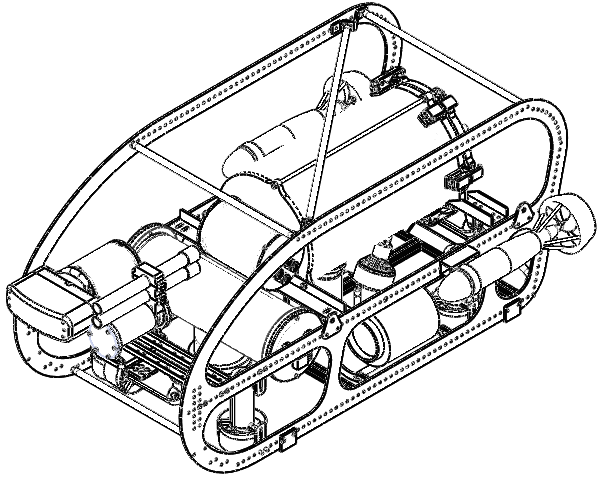
\includegraphics[width=2.6in]{BBAUV.png}
\caption{BumbleBee AUV 2.0}
\end{figure}

Table \ref{specs} shows the hardware of BumbleBee 2.0.

\begin{table}[h]
\centering
\begin{tabular}{|p{0.8in}|p{2.0in}|}
\hline
\textbf{Weight} & 48 kg \\ \hline
\textbf{Dimensions} & 0.7m X 1.1m X 0.5m \\ \hline
\textbf{\begin{tabular}[c]{@{}l@{}}Single Board\\ Computer\end{tabular}} & \begin{tabular}[c]{@{}l@{}}Core i7 - 3610QE\\ Aaeon EMB-QM77\\ 8GB DDR3 RAM\\ 512GB SATA3 SSD\end{tabular} \\ \hline
\textbf{\begin{tabular}[c]{@{}l@{}}Embedded\\ Systems\end{tabular}} & \begin{tabular}[c]{@{}l@{}}Arduino Mega 2560\\ Xilinx Spartan-3 on NI sbRIO 9602\end{tabular} \\ \hline
\textbf{Propulsion} & \begin{tabular}[c]{@{}l@{}}6 SeaBotix BTD150\\ 2 VideoRay Surge Thrusters\end{tabular} \\ \hline
\textbf{Navigation} & \begin{tabular}[c]{@{}l@{}}Teledyne RDI Explorer DVL\\ Sparton AHRS-8 IMU\\ Pressure/Depth Sensor\end{tabular} \\ \hline
\textbf{\begin{tabular}[c]{@{}l@{}}Vision \\ Sensors\end{tabular}} & \begin{tabular}[c]{@{}l@{}}AVT Guppy Pro 1394b\\ Microsoft Lifecam Cinema\end{tabular} \\ \hline
\textbf{Sonar} & \begin{tabular}[c]{@{}l@{}}BlueView P450 Imaging Sonar\\ 4 Teledyne Reson TC4013 Hydrophones\end{tabular} \\ \hline
\textbf{Manipulators} & Festo Pneumatics Systems \\ \hline
\textbf{Power Supply} & 22.2V 7800mAh LiPo Battery (x2) \\ \hline
\textbf{Underwater Connectors} & SubConn Micro and Low Profile Series \\ \hline
\textbf{\begin{tabular}[c]{@{}l@{}}Software\\ Architecture\end{tabular}} & \begin{tabular}[c]{@{}l@{}}Robot Operating System (ROS)\\ Debian GNU/Linux x64\end{tabular} \\ \hline
\end{tabular}
\caption{BumbleBee AUV 2.0 Specifications} 
\captionsetup{justification=centering}
\label{specs}
\end{table}

\section{Mechanical Sub-system}
The 2013-2014 vehicle, BumbleBee 2.0, features a complete redesign from the previous vehicle. This design improvement, inspired by industrial ROVs (Remote Operated Vehicles), has reduced the overall weight to 48 kg while allowing for more sensors and actuators. At the same time, this increases robustness and modularity to aid disassembly during troubleshooting. \\

The key features of the mechanical system are the frame, hull, thrusters configuration, manipulators and the external housings. Custom battery pods have been built to accommodate the newer and larger battery management system. \\

All aluminum components of the mechanical subsystem are fabricated from 6061-T6 aluminum. They are then hard anodized and sealed for maximum corrosion resistance, electrical insulation and scratch resistance. FEA (Finite Element Analysis) is employed for weight optimisation.

\begin{figure}[h]
\centering
\includegraphics[width=3.5in]{AUVview.png}
\captionsetup{justification=centering}
\caption{View of AUV: left, front, right, back}
\end{figure}

\subsection{Frame}
With the help from Cititech industrial engineering, the frame is made by laser cutting sheet aluminum and is bolted together with hardware from Bossard. The robust and rigid frame encompasses all components and protects them from impact. Its precisely determined drill pattern allows for easy adjustment of component positions.

\subsection{Hull}
BumbleBee's hull is made of a standard size acrylic tube featuring end caps that are fabricated by CNC (Computer Numerical Control) machining of aluminum. Sealing is achieved by using the six Southco draw latches to compress an O-ring between the end caps. The draw latches allow for rapid disassembly of the hull. This improvement over the previous bolted flange design eases access to the electronics within the hull, facilitating troubleshooting of components. The end caps are sealed to the acrylic tube via a radial seal.

\begin{figure}[h]
\centering
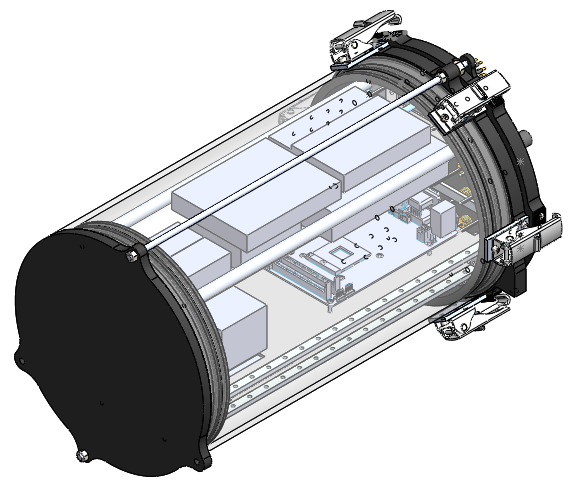
\includegraphics[width=2.5in]{HullFrontview.png}
\caption{Hull, Front View}
\end{figure}

\begin{figure}[h]
\centering
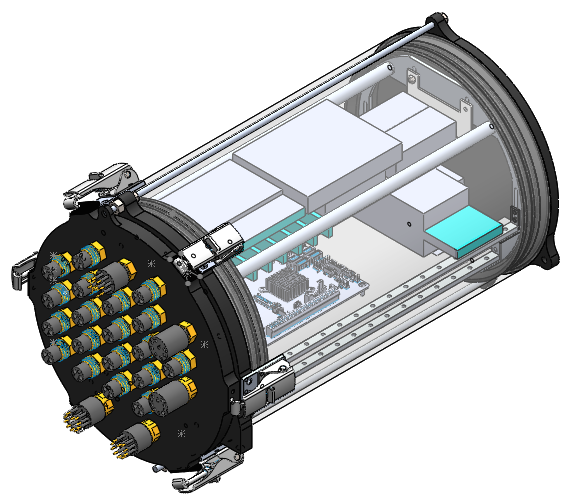
\includegraphics[width=2.5in]{HullBackview.png}
\caption{Hull, Back View}
\end{figure}

A valve on the hull allows it to be pressurized and also monitors any drops in pressure. This feature allows the hull to be tested for any leaks before the vehicle is submerged in water. A pressure is maintained about 120 kPa during operations. Any pressure drop indicates a hull leak, which would activate the leak sensor. The leak alert is propagated to the BumbleBee Control Panel which displays a warning. Extensive pressure testing of the hull was conducted at Hallin Marine's pressure testing facility and the hull is rated to a depth of 40 meters. 

\subsection{Thrusters Configuration}
Six SeaBotix and two VideoRay thrusters have been mounted on the vehicle to provide six degrees of freedom. Movement in the heave and the sway are controlled by four and two SeaBotix thrusters respectively. Surge movement is guided by the two horizontally placed VideoRay thrusters. \\

The VideoRays are chosen as the surge thrusters to overcome the 71 N drag force encountered during high forward thrust. The VideoRay pair provides 96 N of thrust as compared to 58 N from a SeaBotix pair. Despite the large forward force provided by the VideoRays, they have coarser speed control and lower resolution than the SeaBotixs. Hence they are used for forward (surge) movement while the six SeaBotixs are employed for precision movement in the other axes. 

\subsection{External Enclosures}
BumbleBee's external enclosures house the electrical systems located outside the main hull. These comprises the DVL (Doppler Velocity Log) housing, camera housing, the hydrophones enclosure and the battery pods. \\

\subsubsection{DVL Housing}
The DVL housing was fabricated by welding 6061 aluminum tubes into a $T$ structure. The vertical tube houses the sensor head while the horizontal tube houses the electronic box. SubConn low profile bulkheads are used to provide an electrical connection. The end caps are sealed against the tube with a double O-ring radial seal. \\

\begin{figure}[h]
\centering
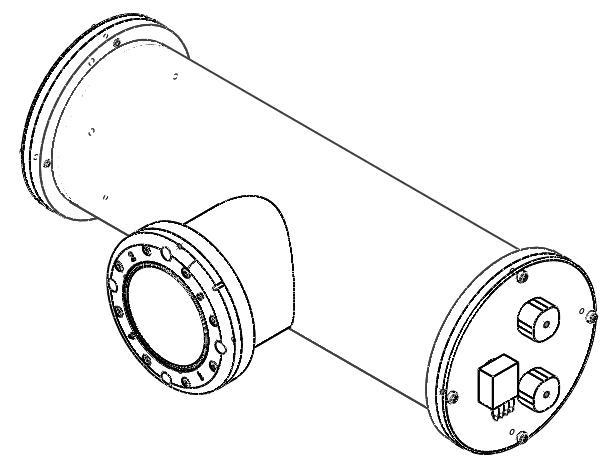
\includegraphics[width=2.3in]{DVLHousingbnw.png}
\caption{DVL Housing}
\end{figure}

\subsubsection{Battery Pods}
The battery pods consist of acrylic tubes epoxied to off-the-shelf screw on/off end caps that are integrated with O-ring seals. The pods feature titanium pressure relief valves from DeepSea Power and Light. This safety feature prevents an explosion in the event of pressure build-up in the battery pod from overcharging of the LiPo battery housed in the pod. SubConn MCBH16F and MCBH8F underwater connectors are attached to the pods to serve as power lines and balancing leads for the LiPo batteries respectively.

\subsection{Manipulators}
The vehicle's manipulators comprises of a pair of grabbers, torpedo launchers and a marker dropping mechanism, all of which are fabricated by 3D printing. The grabber design has been modified from the previous year's to be more compact for better integration into the vehicle. The torpedo design incorporates an O-ring to create a pressure build-up necessary to launch the torpedo. A ball dropping mechanism is designed for the marker task. This mechanism can hold up to four balls at once and drop them individually. The manipulators are actuated by a Festo Singapore pneumatic system stored in a 13 cubic inch Ninja Paint ball tank.

\begin{figure}[h]
\centering
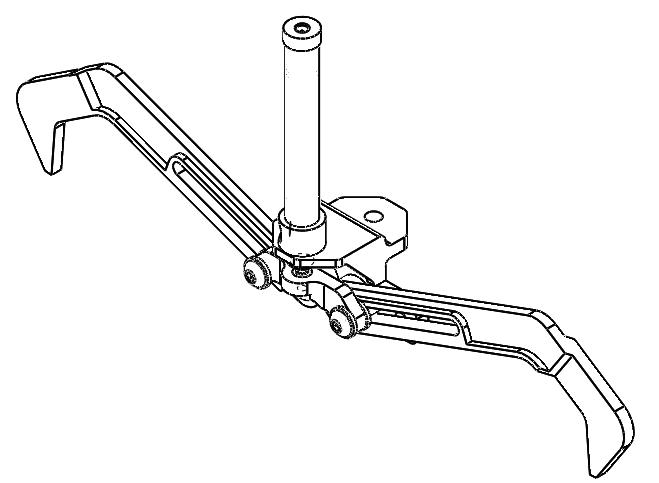
\includegraphics[width=2.1in]{Grabber.png}
\caption{Grabber}
\end{figure}

\begin{figure}[h]
\centering
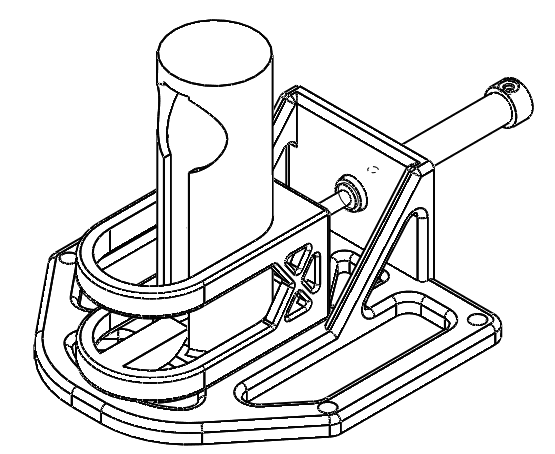
\includegraphics[width=2.1in]{Dropper.png}
\caption{Dropper}
\end{figure}

\section{Electrical Sub-system}
The electrical system comprises of the power, sensors and actuators and the computer subsystems. The previous OpenUPS power subsystem has been replaced with the integration of Battery Management Boards. The sensors and actuators have been redesigned and additional ones are integrated. The main computer board hosts a quad core i7 processor for fast multicore software processing. The components are integrated on a single multi-level rack fitted into a single hull. 

\subsection{Power System}
The vehicle is powered by two 7800 mAh LiPo (lithium polymer) batteries extending testing time to approximately 150 minutes before requiring a recharge. \\

\subsubsection{Power Monitoring and Management}
Each LiPo battery is installed into a battery pod which allows for both charging and discharging. Within the pod, the batteries are connected to PMB (Power Monitoring Boards) which monitor vital power statistics such as current, cell voltage and capacity. The custom fabricated PMB has been designed to withstand a maximum current of 30 A. This system allows tracking of power statistics of the batteries and is more reliable than the previous off-the-shelf OpenUPS system. \\

A battery charging box has been designed for quick deployment of mobile charging stations. This battery charging box supports parallel charging of two battery pods of up to 25 A per channel at one go. \\

\begin{figure}[h]
\centering
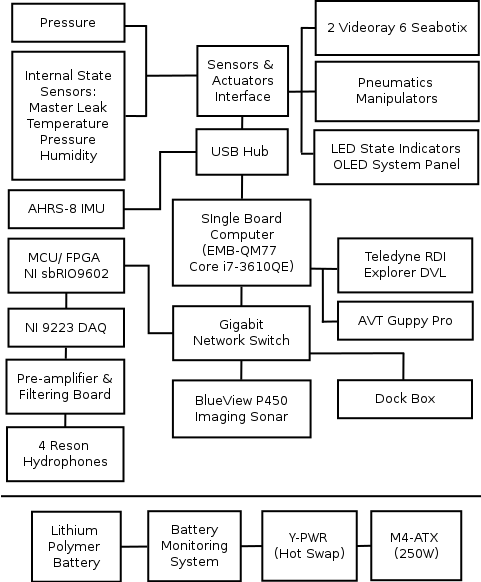
\includegraphics[width=3in]{diagram.png}
\caption{Electrical System Block Diagram}
\captionsetup{justification=centering}
\end{figure}

\subsubsection{Power Distribution}
Power distribution is simplified by BMB (Battery Management Boards) that replaces the OpenUPS of the previous vehicle. This change improves the power efficiency without the OpenUPS step down regulator and has lesser points of failure. Diagnostics are streamed from the PMB via serial connection to the SBC  (Single Board Computer). The power system utilizes a M4 ATX to regulate power in order to generate three voltage rails to power up the SBC and the sensors and actuators. A Y-PWR provides hot-swap capabilities for the batteries without shutting down the motherboard. 

\subsection{Sensors and Actuators}
BumbleBee 2.0 presents a redesigned and custom fabricated PCB (Printed Circuit Board) for the sensors and actuators shield. The Arduino Mega 2560 microcontroller developmental board is based on the previously used ATMega 2560 microcontroller. The previous shield design was continued for the quick swap of microcontroller crucial for modular debugging during port or component damages. \\

\begin{figure}[h]
\centering
\includegraphics[width=3in]{mega2560.png}
\caption{Sensors and Actuator Board design}
\captionsetup{justification=centering}
\end{figure}

New sensors such as internal pressure and humidity sensors are added to the current suite of the AHRS-8 IMU, depth and temperature sensors. This board also interfaces the six SeaBotix thrusters and the pneumatic manipulators. The current thrusters are enhanced by including actuator controls to the electronic speed controllers operating on the two VideoRay surge thrusters. \\

In addition, LED strips are integrated as state indicators, while a TFT LCD screen display provide visual feedback on the system sensor status. These indicators are especially useful during autonomous runs for understanding the vehicle's current state.

\subsection{Navigational Sensors}
\subsubsection{Sparton AHRS-8 IMU}
The Sparton AHRS-8 IMU (Inertia Measurement Unit) provides critical inertial data at a rapid rate of 100 Hz. The IMU's proprietary algorithms ensure the output of correct data despite the presence of electromagnetic interference generated by the BumbleBee's suite of electronics and
thrusters. \\

\subsubsection{Teledyne RDI Explorer DVL}
The DVL (Doppler Velocity Log) is an active sonar system that tracks the velocity of
the instrument via a four-beam solution directed at 30 degrees nominal from the
sensor's ceramic head. The velocity readings obtained are combined with tilt and altitude measurements, then resolved into the three orthogonal $x$, $y$ and $z$ axes via a least squares fit solution. These resolved readings are further filtered through a direct three-degree of freedom Kalman filter, which serves to attenuate noise. The calculations outputs a more accurate positional coordinate of the vehicle. \\ 

\subsubsection{Navigation}
The data provided by the navigational sensors are fused together via
trigonometric equations to generate a global position vector. The odometric data obtained from this vector allows precise navigation to a given spatial coordinate.

\subsection{Computer System}
BumbleBee's software system is powered by an Intel Core i7-3610QE quad core processor on an Aaeon PCM-QM77 motherboard along with a 512 GB SATA SSD (Solid State Drive). This upgrade from the previous 16 GB SSD accommodates more software data and rosbag data collected. \\

A USB hub interfaces the embedded sensors and actuators as well as other serial devices, i.e. two PMBs and the AHRS-8. The imaging sonar is connected via Ethernet with a PoE (Power over Ethernet) connection to the SBC, dedicating imaging sonar bandwidth to the main computer. VGA and USB ports are exposed to allow external debugging of the software systems. \\

The computer is connected to dockside via a 100 Mbps Ethernet tether. The vehicle is networked to a Gigabit switch that connects to NI sbRIO 9602 and surface router. A wireless transceiver is integrated as a secondary redundant link, deployed when the wired Ethernet communication fails. 

\subsection{Control System}
Six PID (Proportional Integral Derivative) control loops are tuned using a UI developed by the software team to control the vehicle's six degrees of freedoms. The PID controllers are designed with the following considerations:

\begin{itemize}
\item {Low pass filter for the derivative component to reduce the exponential effects on sensor noise}
\item {Variable period time sampling for more accurate integral and differential computation}
\item {Weighted set points to reduce transient effects in set point changes}
\item {Integrator windup protection for when actuators are unable to fulfill the PID Controller requirements \\ }
\end{itemize}

The PID control loops have been improved for dynamic allocation of actuator limits, allowing greater output in specific degree of freedoms. Velocity controllers for the surge and sway domains have been implemented for more precise maneuvering of the vehicle during mission runs.

\begin{figure}[h]
\centering
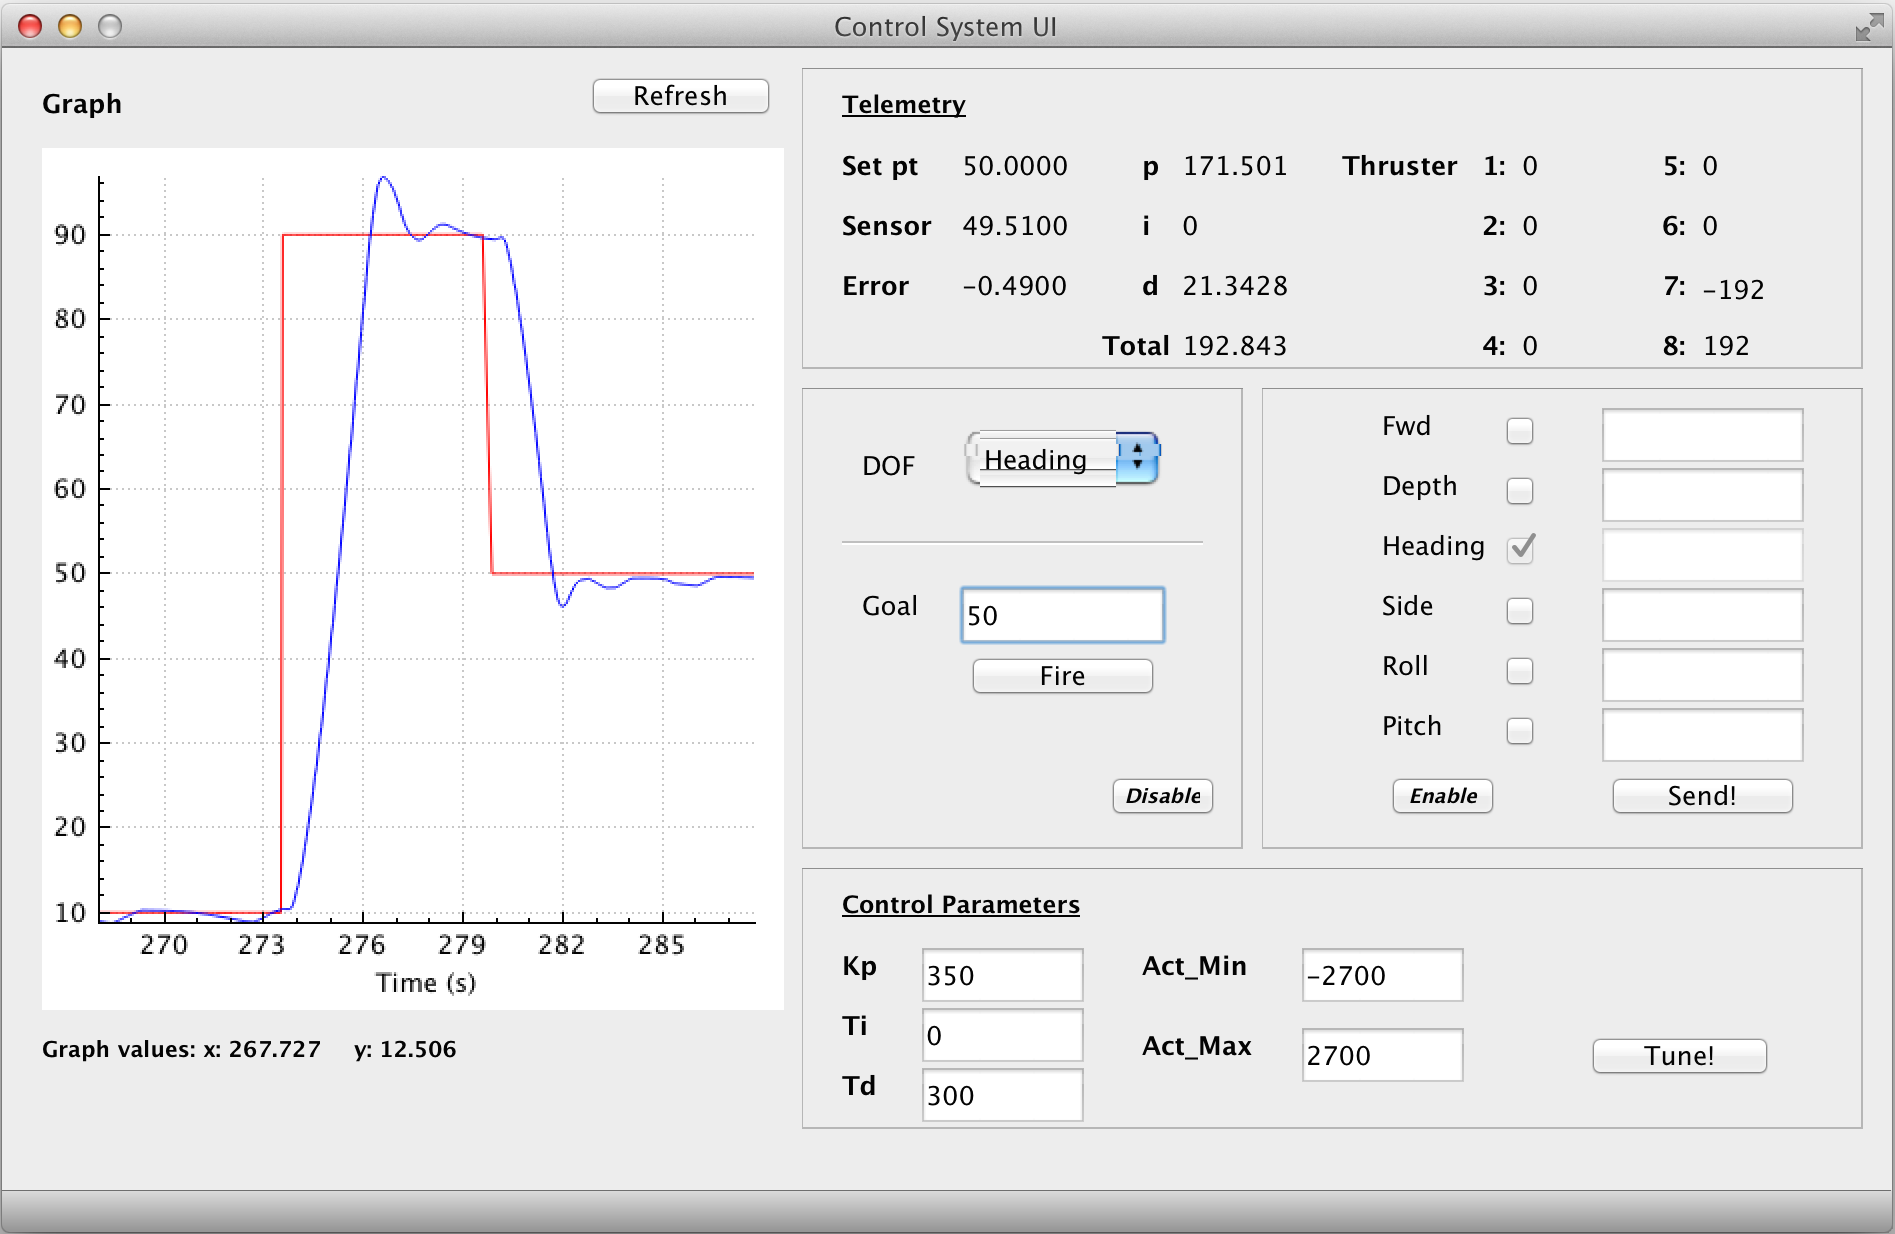
\includegraphics[width=3in]{controlui.png}
\caption{PID tuning UI}
\captionsetup{justification=centering}
\end{figure}

\section{Acoustic Sub-system}
BumbleBee's acoustic sub-system has four Teledyne hydrophones, integrated with custom fabricated analog and digital boards. A high-resolution MUSIC (MUltiple SIgnal Classification) algorithm is used to localise the acoustic pinger. 

\subsection{Hydrophone Array}
With the MUSIC beamforming algorithm, the inter-element spacing $d$ between each hydrophone element should not exceed half of the carrier wavelength to avoid spatial aliasing. The compact 9.5 mm Teledyne TC 4013 hydrophone can achieve this in a square array with $d$ of 1.5 cm. This hydrophone mount is designed on SolidWorks and fabricated precisely using laser-cutting technology.

\begin{figure}[h]
\centering
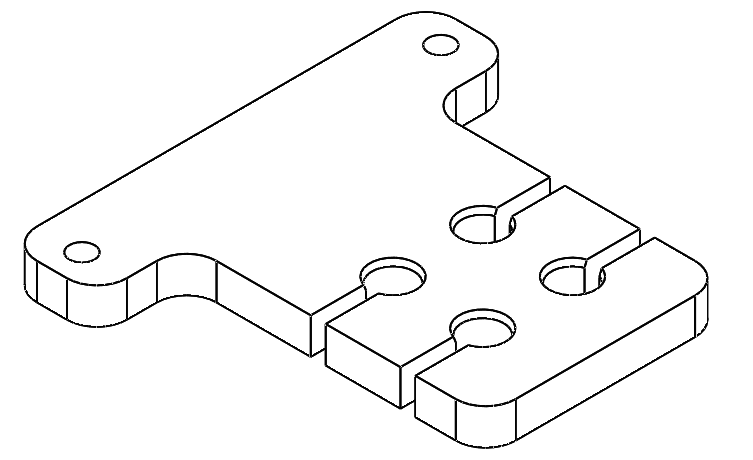
\includegraphics[width=1.8in]{hydrophonemount.png}
\caption{Hydrophone Mount}
\end{figure}

\subsection{Analog and Digital Boards}
An analog pre-amplifer and bandpass filter board is fabricated for signal amplification and noise attenuation. The analog signal is digitally sampled at 250 kS/s by a NI (National Instruments) NI9223 Analog Input Module (DAQ). Array signal processing algorithms are programmed with LabVIEW 2012 on NI sbRIO NI9206 (FPGA). The FPGA transmits the computed FFT (Fast Fourier Transform) information through UDP to the SBC for application of the MUSIC algorithm.

\subsection{Algorithm}
The sampled signal is passed into an elliptic 10th order band pass filter with a center frequency set to the pinger's. This digital filter has a 3 dB bandwidth of 5 kHz. The start of each ping must be correctly identified to compute information on its phase. This is estimated with peak and dynamic threshold detection as the received power varies with distance. \\

Only the initial segment of the ping is extracted for post processing. This avoids phase distortion when multipath reverberation effects set in at a later stage. The amount of samples extracted is defined by a FFT size  determined by extensive experimentation. FFT-operations are performed on the extracted ping to verify that the identified signal falls within the frequency range of the pinger. If the signal falls within the defined frequency range, the complex numbers (FFT points) associated with the peaks of the power spectrum are extracted. These FFT points are used to compute the covariance matrix used in the MUSIC algorithm. \\

The spatial covariance matrix is computed over three pings. The eigenvectors corresponding to the signal and noise subspaces are obtained from eigen-decomposition of the spatial covariance matrix. The MUSIC algorithm searches for a set of azimuth $\theta$ and elevation $\phi$ where the array steering vector $\alpha(\phi,\theta)$ is the most orthogonal to the noise eigenvectors $V_n$. The direction of the pinger is indicated by the maximum point of $P_{music}$ derived from the 2-D search in $\theta$ and $\phi$.

\begin{equation} 
P_{music} = \frac{\alpha^H(\phi,\theta)\alpha(\phi,\theta)}{\alpha^H(\phi,\theta)V_nV_n^H\alpha(\phi,\theta)V_n} 
\end{equation}

\begin{equation}
\alpha(\phi,\theta) = \begin{bmatrix}
e^{\frac{j2 \pi r} {\lambda} sin(\phi)cos(\theta-\sigma_{0})}\\
e^{\frac{j2 \pi r} {\lambda} sin(\phi)cos(\theta-\sigma_{1})}\\
e^{\frac{j2 \pi r} {\lambda} sin(\phi)cos(\theta-\sigma_{2})}\\
e^{\frac{j2 \pi r} {\lambda} sin(\phi)cos(\theta-\sigma_{3})}\\
\end{bmatrix}
\end{equation}

\begin{figure}[h]
\centering
\includegraphics[width=2.8in]{MUSICplot.png}
\captionsetup{justification=centering}
\caption{Direction of Pinger: $\theta=269^\circ,\phi=20^{\circ}$ }
\end{figure}

\section{Software sub-system}
Bumblebee's software system consists of the mission planner and the vision subsystems to complete the competition courses. The software system is built upon Debian GNU/Linux x64, providing multicore processing for the vision, control and mission systems. \\

Built on the last year's architecture, the software stack is based on the ROS (Robot Operating System) Software Framework by Willow Garage. The ROS distribution has been upgraded from Fuerte to Hydro. Each software unit is a ROS node, and all communication, data acquisition and publishing are done through the ROS architecture. The software stack has been further modularised to allow experimentations and quick reconfiguration on-site. Highly customisable interfaces have been developed in Python to facilitate vision tuning. Locomotion of the vehicle is achieved using the action servers and clients based on the ROS actionlib API. 

\subsection{Mission Planner} 
Vehicle dynamics during mission runs is controlled by the mission
planner, which directs task nodes, controls trajectory between tasks and manages 
time. The mission planner is written in Python and utilizes a finite state 
machine structure. \\

The highly modular software architecture complements the functionality of the mission planner. The mission planner's multi-threaded structure allows for simultaneous execution of mission tasks and watch states that serve to keep track of the mission and task statuses. It is coupled with extensions for execution and cleanup of arbitrary scripts on the fly. The mission planner also manages contingency states to allow for recovery via the saved waypoints during the mission run. \\

Mission runs can be dynamically built from user input, providing an option to test task nodes independently in addition to a full mission test. The vehicle status is consistently checked and an alert is sounded in the event of an irrecoverable component failure. 

\subsection{Vision}
BumbleBee’s vision processing system consists of modular communication, movement and vision filtering packages that can be combined and tuned to complete each mission task. Each vision processing unit runs as a separate ROS node and is responsible for a single task, providing both movement through ROS SMACH state machines, and vision output, while cooperating with other units running in parallel through mission planner. BumbleBee’s front and bottom facing Microsoft Lifecam Cinema cameras provide sufficient visual feedback for the vision processing system. Improved vision algorithms are applied for better identification of the required objects. \\

\subsubsection{Vision Processing}
The vision nodes receive image input from the cameras in the Bayer encoded bgr8 format through the ROS protocol. The ROS images are converted to OpenCV images via the ROS cvBridge. To deal with changing water and lighting conditions, various image enhancement techniques such as image sharpening, white balancing, gray world and adaptive thresholding values are applied to obtain better image contrast. \\

A combination of vision filters are used to detect, classify and track objects. These include HSV colour thresholding, contour detection and Hough transforms provided by the OpenCV computer vision library. The vision processing code is written in Python and an annotated processed image is published as a ROS image. Centroid calculation is performed using Hu moment analysis to align the camera's center with the centroid identified. The centroid is tracked at each frame while the vehicle maneuvers into position, before performing further object identification and manipulation to complete the task at hand. \\

\begin{figure}[h]
\centering
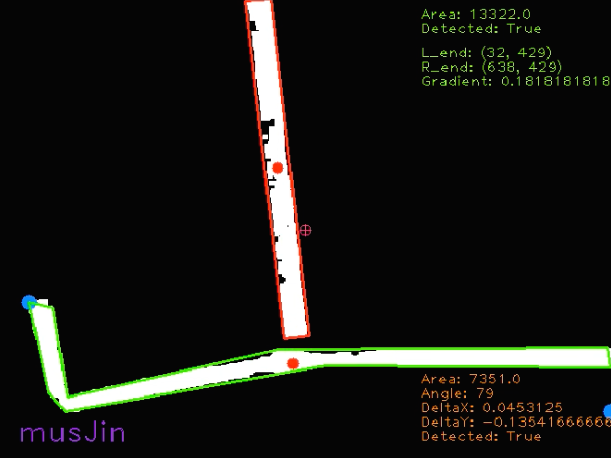
\includegraphics[width=3.0in]{manu_paper_filter.png}
\caption{Annotated image \\ of maneuvering task}
\captionsetup{justification=centering}
\label{fig:image_manu}
\end{figure}

\subsubsection{Vision Tuning}
Vision tuning systems are developed using PyQt for experimentation of vision processing parameters at real time. These systems receive a live update from the cameras and the vision processing units and provide analysis of image statistics such as colour histograms. The ROS dynamic reconfigure tool is also used to quickly adjust parameters. These configuration parameters are stored until the next system reboot.  

\begin{figure}[h]
\centering
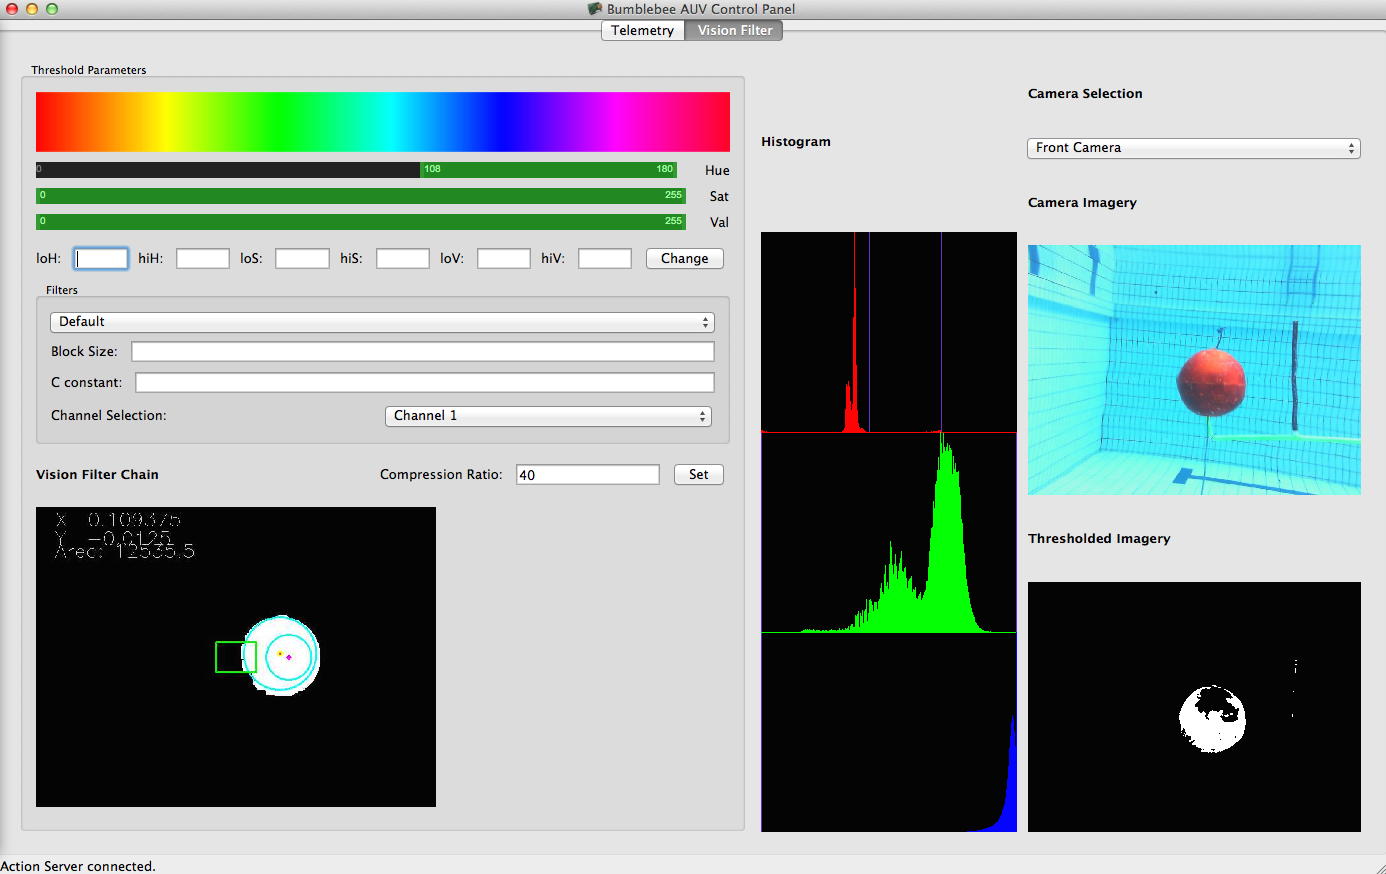
\includegraphics[width=3.5in]{controlpanel.png}
\caption{Threshold parameters tuning UI}
%\captionsetup{justification=centering}
\end{figure}

\subsection{Imaging Sonar}
BumbleBee 2.0 incorporates a multi-beam forward facing BlueView P450 active imaging sonar to extend the field of view beyond the camera's in order to enhance mission effectiveness. The sonar operates at a frequency of 450 kHz with a 45 degrees field-of-view, yielding a maximum range of 250 m. Its 10 Hz refresh rate serves to assist in completing the front camera vision tasks.

\begin{figure}[h]
\centering
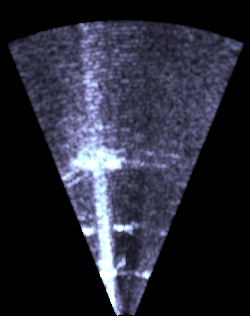
\includegraphics[height=2.3in]{sonarimage.png}
\caption{Sonar Image at 6m}
\captionsetup{justification=centering}
\end{figure}

\subsection{Vehicle logging}
The BumbleBee Control Panel displays telemetry and camera information, enabling monitoring of sensors and actuator data for system analysis during practice runs. This control panel has been enhanced and integrated to interface with the information published by the new electrical system. 

\begin{figure}[h]
\centering
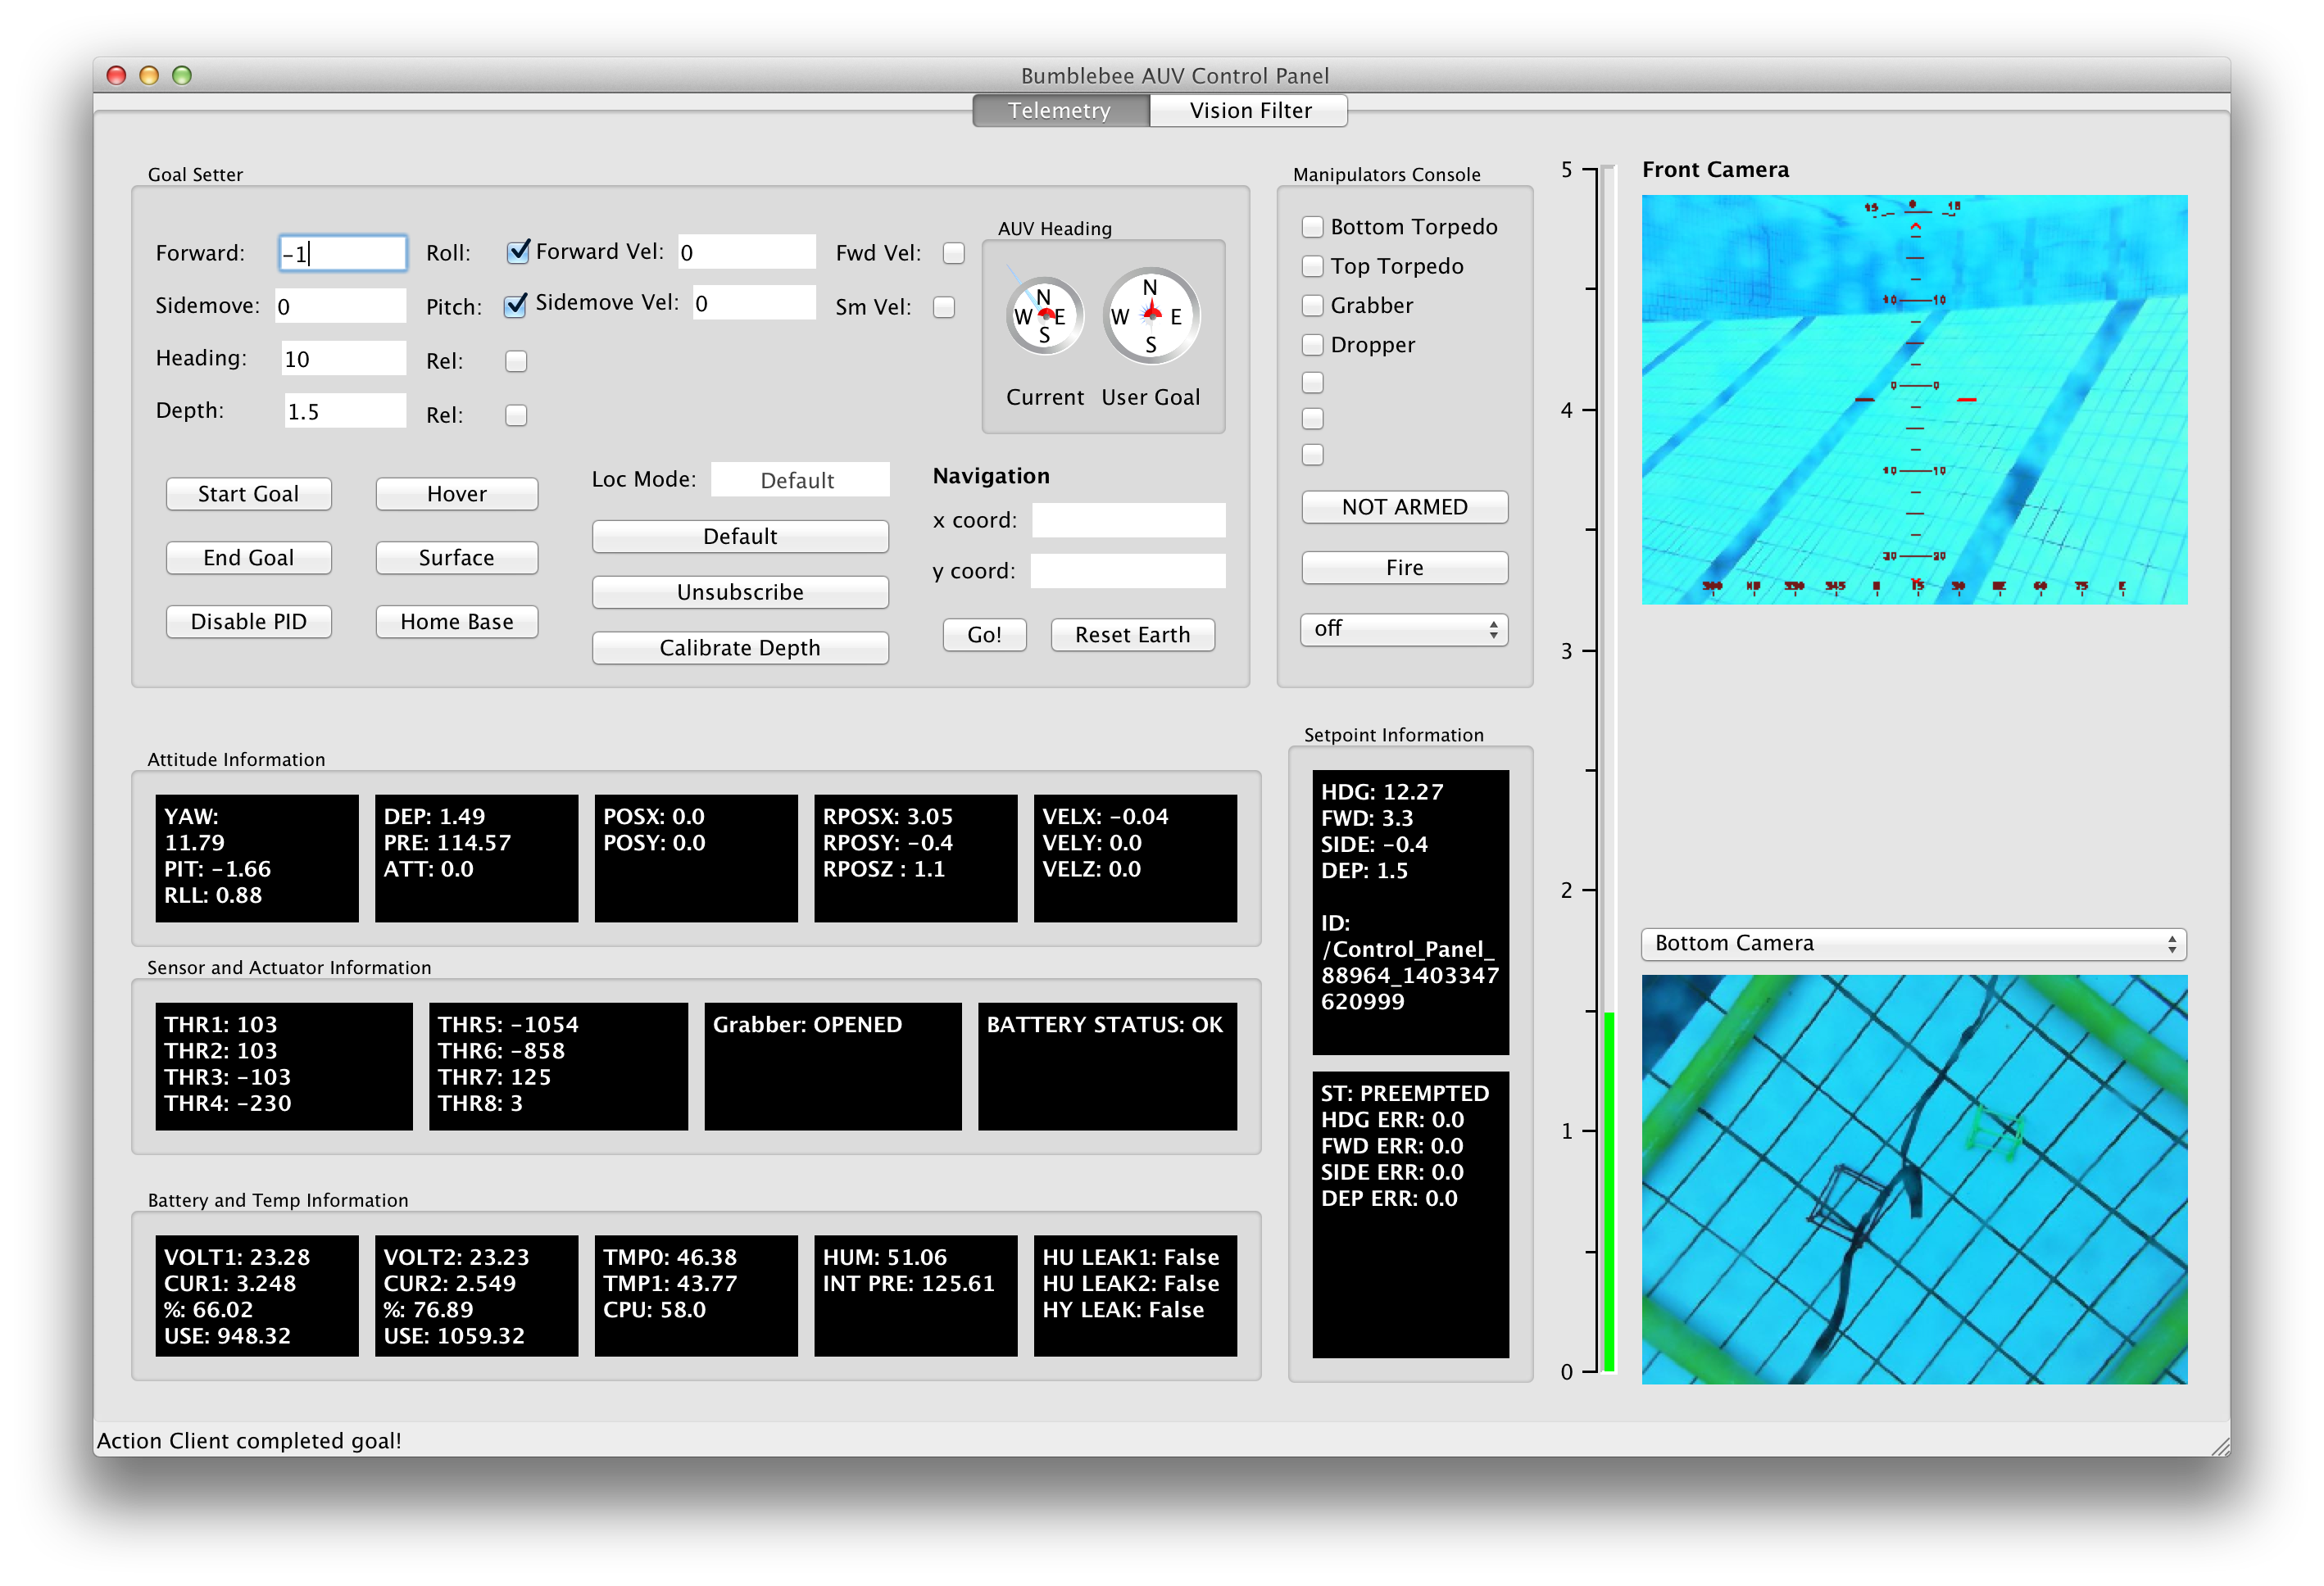
\includegraphics[width=3.8in]{telemetry.png}
\caption{BumbleBee control panel}
\captionsetup{justification=centering}
\end{figure}

The ROS logging system is used to capture telemetry and video information, and log messages during both tethered and autonomous runs. The data is captured in .bag files in the form of ROS messages. The rosbag playback utility is used to allow post-processing to improve the algorithms and system.

\section{Vehicle Status and Testing}
BumbleBee 2.0 has been undergoing extensive pool tests since February 2014. Prior to the integration of the vehicle, the mechanical subsystem was thoroughly leak tested; the electrical components were bench tested; the software subsystem was constructed and tested on recorded data from previous runs. In preparation for RoboSub 2014, pool tests are being conducted at Queenstown Swimming Complex almost daily.

\section{Conclusion}
BumbleBee 2.0 is a modular Autonomous Underwater Vehicle designed for accomplishing the vision and acoustic tasks for RoboSub and the Singapore AUV Challenge. Significant upgrades have been made from the previous vehicle, including a complete redesign of the mechanical system, better integration of sensors and actuators and further improvements of the software suite. Future work includes further development of the electrical systems architecture; integrating TDOA (Time Difference of Arrival) with beamforming techniques for acoustic localisation; designing more interactive software to display telemetry data; and developing a more robust vision suite for adapting to different conditions. \\

\begin{figure}[h]
\centering
\includegraphics[width=3.5 in]{auv.png}
\caption{BumbleBee 2.0}
\captionsetup{justification=centering}
\end{figure}

\begin{figure}[h]
\centering
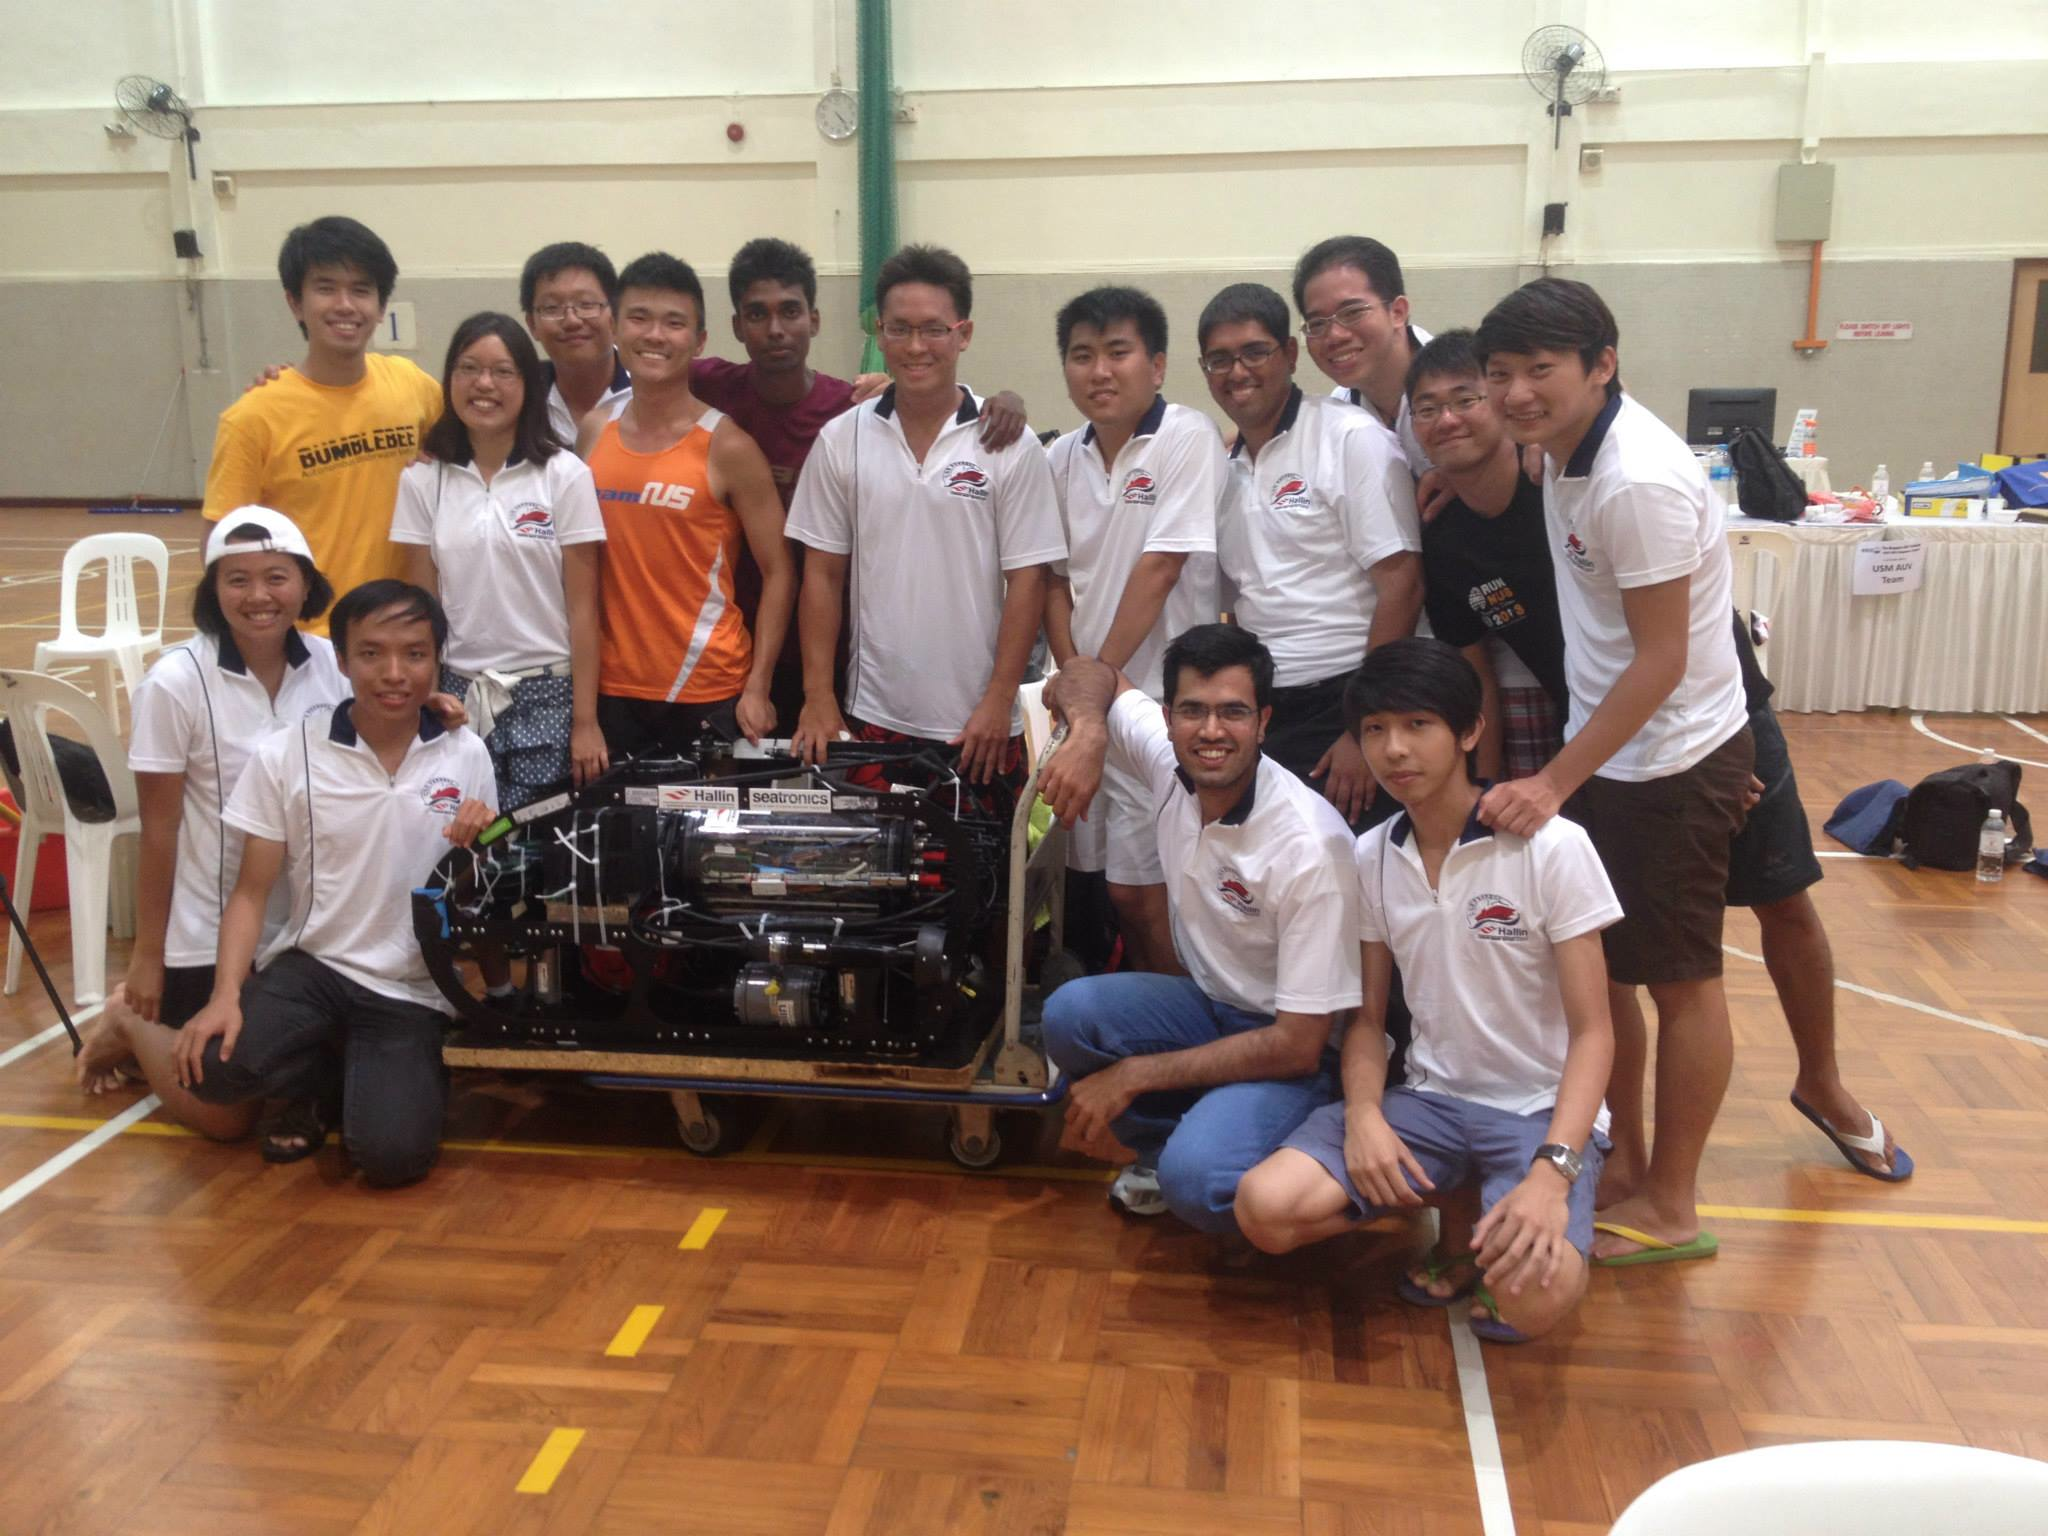
\includegraphics[width=3.5 in]{team.png}
\caption{Team BumbleBee 2014}
\captionsetup{justification=centering}
\end{figure}


\section*{Acknowledgements}
Team BumbleBee would not have been where it is today without the following people and we would like to thank them for giving us the chance to compete in RoboSub:

\subsection*{Title Sponsor Hallin Marine}
For their sponsorship towards the team for a second year running and flying the team across the globe to participate in RoboSub.

\subsection*{Platinum Sponsors}
\subsubsection*{NUS} for equipment procurement, on-campus accommodation, cash sponsorship and academic and technical support.

\subsubsection*{Seatronics Group} for the continued loan of Workhorse DVL, BlueView Imaging Sonar and underwater connectors.

\subsection*{Gold Sponsors} 
Cititech Engineering, National Instruments, Festo

\subsection*{Silver Sponsors} 
IKM, Kentronics Engineering, Teledyne Reson, Allied Vision Technologies, Edmund Optics, Sparton, Evernote

\subsection*{Bronze Sponsors}
Sterling Comm Intl Pte Ltd, Aaeon Technologies 

\subsection*{Equipment discounts and other partners} 
Deep Sea Power and Lights, Southco, Bossard, Pololu Robotics, Tekin, Digikey, Aztech, SeaBotix, Advanced Marine and Acoustic Research Lab

\end{document}